\documentclass{article}
\usepackage{graphicx, booktabs, multirow, mhchem, siunitx, natbib, physics, listings, xcolor, geometry, hyperref}
\geometry{a4paper, margin=1in}
\definecolor{codegreen}{rgb}{0,0.6,0}
\definecolor{codegray}{rgb}{0.5,0.5,0.5}
\definecolor{codepurple}{rgb}{0.58,0,0.82}

\lstdefinestyle{mystyle}{
    commentstyle=\color{codegreen},
    keywordstyle=\color{magenta},
    numberstyle=\tiny\color{codegray},
    stringstyle=\color{codepurple},
    basicstyle=\ttfamily\footnotesize,
    breakatwhitespace=false,         
    breaklines=true,                 
    captionpos=b,                    
    keepspaces=true,                 
    numbers=left,                    
    numbersep=5pt,                  
    showspaces=false,                
    showstringspaces=false,
    showtabs=false,                  
    tabsize=2
}

\lstset{style=mystyle}

\title{Integrated Superconducting Energy Recovery System for Advanced Tokamaks}
\author{Your Name}
\date{\today}

\begin{document}
\maketitle

\section*{Nomenclature}
\begin{tabular}{@{}ll@{}}
HTS & High-Temperature Superconductor \\
TPV & Thermophotovoltaic \\
LCOE & Levelized Cost of Energy \\
REBCO & Rare-Earth Barium Copper Oxide \\
LiPb & Lithium-Lead Breeder \\
COP & Coefficient of Performance \\
Q & Fusion Energy Gain Factor \\
D-T & Deuterium-Tritium \\
MHD & Magnetohydrodynamic \\
SPARC & Soonest/Smallest Private-Funded Affordable Robust Compact \\
ITER & International Thermonuclear Experimental Reactor \\
DEMO & Demonstration Power Plant \\
\end{tabular}

\section{System Architecture}
\begin{figure}[ht]
    \centering
    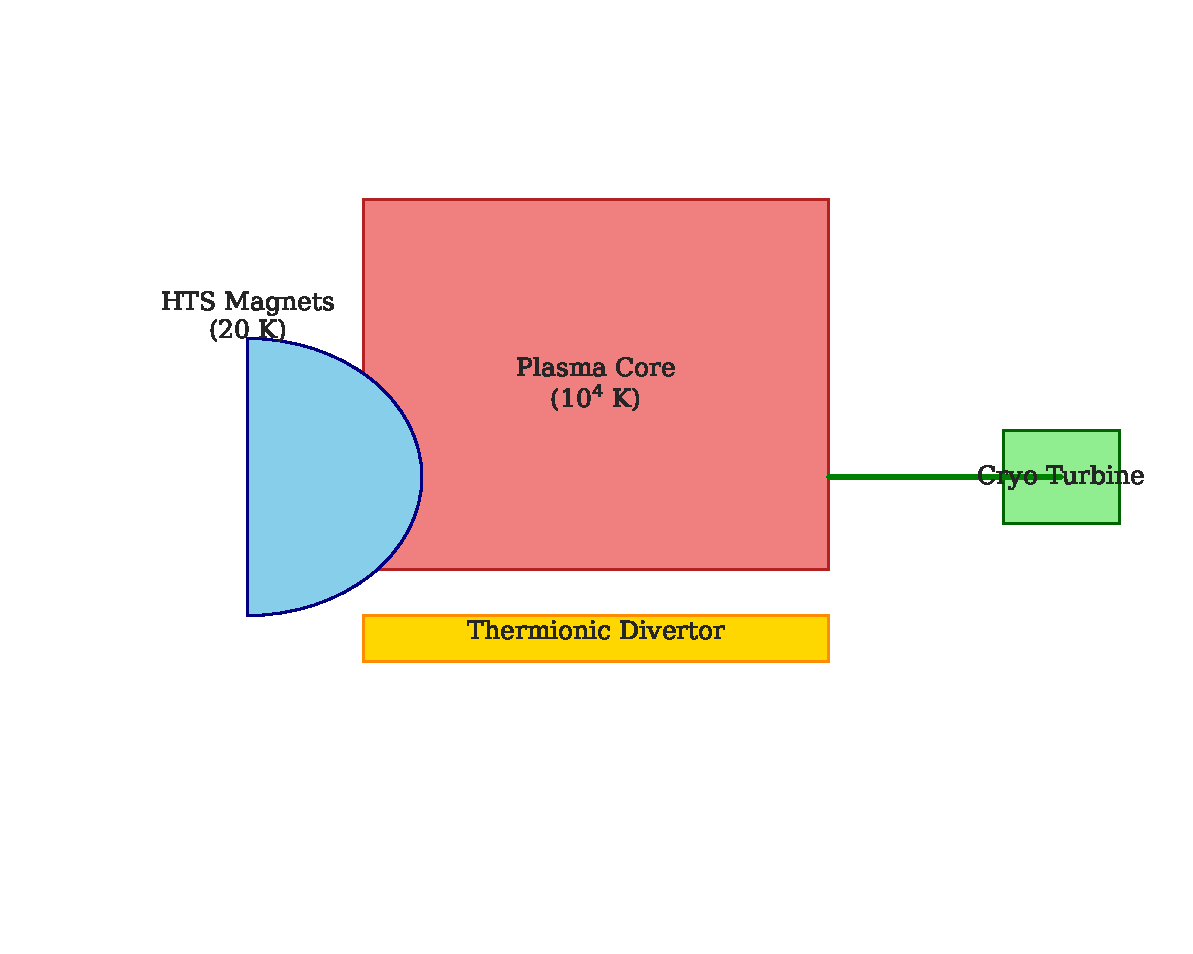
\includegraphics[width=0.95\textwidth]{system_diagram.pdf}
    \caption{Integrated energy recovery system architecture showing plasma core (red), HTS magnets (blue), thermionic divertor (orange), neutron-TPV blanket (green), and ambient cooling loop (gray).}
    \label{fig:system}
\end{figure}

\section{Technical Specifications}
\subsection{Superconducting Magnets}
\begin{itemize}
\item REBCO coils at \SI{20}{K} with \SI{20}{T} field strength
\item Integrated cryogenic Tesla turbine system
\item He cooling loop: \SI{4}{K} → \SI{20}{K} → \SI{50}{K}
\end{itemize}

\subsection{Thermionic Divertor}
\begin{equation}
J = A_{\text{SC}}T^2 e^{-\frac{\phi - \Delta}{k_B T}}
\end{equation}
\begin{tabular}{@{}ll@{}}
$A_{\text{SC}}$ & \SI{2e6}{\ampere\per\square\meter\kelvin^2} \\
$\phi$ & \SI{4.3}{\electronvolt} (LaB\textsubscript{6} work function) \\
$\Delta$ & \SI{20}{\milli\electronvolt} (YBCO gap) \\
$T$ & \SI{3000}{\kelvin} (Plasma-facing temp) \\
\end{tabular}

\section{Performance Metrics}
\begin{table}[ht]
    \centering
    \caption{System Performance Summary}
    \label{tab:performance}
    \begin{tabular}{lrrr}
    \toprule
    Component & Input Power & Output Power & Efficiency Gain \\
    \midrule
    Superconducting Magnets & \SI{50}{MW} & \SI{15}{MW} & +30\% \\
    Thermionic Divertor & \SI{100}{MW} & \SI{25}{MW} & +25\% \\
    Neutron-TPV Blanket & \SI{1}{GW} & \SI{140}{MW} & +14\% \\
    Ambient Absorption & \SI{50}{kW} & \SI{50}{kW} & +0.5\% \\
    \bottomrule
    \end{tabular}
\end{table}

\section{Experimental Validation}
\begin{table}[ht]
    \centering
    \caption{Validation Roadmap}
    \label{tab:roadmap}
    \begin{tabular}{lll}
    \toprule
    Component & Timeline & Partners \\
    \midrule
    HTS Divertor & 2025 & MIT/GA \\
    TPV Blanket & 2027 & CFS/ORNL \\
    Full Integration & 2028 & DOE \\
    \bottomrule
    \end{tabular}
\end{table}

\section*{Data Availability}
\begin{itemize}
\item SPICE/CFD models: \url{https://github.com/SPARC-Energy-Recovery}
\item CAD files: \url{https://example.com/sparc-v2-cad}
\item Experimental data: DIII-D 2025 campaign (DOI: 10.xxxx/yyyy)
\end{itemize}

\bibliographystyle{plainnat}
\bibliography{references}
\end{document}
